\documentclass[a4paper,12pt,twoside]{scrreprt}
% Autor der Vorlage: Klaus Rheinberger, FH Vorarlberg
% 2017-02-20

%% Hilfe: z.B.
% empfohlener Einstieg: http://latex.tugraz.at/
% https://de.wikibooks.org/wiki/LaTeX-Kompendium:_Schnellkurs:_Erste_Schritte
% https://de.wikibooks.org/wiki/LaTeX-Kompendium:_Schnellkurs
% https://de.wikibooks.org/wiki/LaTeX-Kompendium

%% Pakete:
\usepackage[utf8]{inputenc}
\usepackage[T1]{fontenc}    % Silbentrennung bei Sonderzeichen
\usepackage{graphicx}       % Bilder einbinden
\usepackage[ngerman]{babel} % Deutsche Sprachanpassungen
\usepackage{csquotes}       % When using babel or polyglossia with biblatex, loading csquotes is recommended to ensure that quoted texts are typeset according to the rules of your main language.
\usepackage{acronym}  % für optionales Abkürzungsverzeichnis
\usepackage{eurosym}  % z. B. \EUR{12345,68}
\usepackage[linktocpage=true]{hyperref} % Links z. B. \href{https://www.wikibooks.org}{Wikibooks home}
\usepackage{caption} % Abbildungslegenden
\usepackage{longtable}
\usepackage{ltxtable}
\usepackage{array}
\usepackage{tabularx}
\usepackage{subfiles}
\usepackage{lmodern}
\usepackage{csvsimple}
\captionsetup{format=hang, justification=raggedright}



%% Einstellungen:
\setcounter{secnumdepth}{4}
\setcounter{tocdepth}{4}   % Tiefe der Gliederung im In haltsverzeichnis

%% ERSETZEN VON ECKIGEN KLAMMERN:
% Ersetzen Sie den Text in den eckigen Klammern!

\begin{document}

    % Titelblatt:
    % \newpage\mbox{}\newpage
    \cleardoublepage   % force output to a right page
    \thispagestyle{empty}
    \begin{titlepage}
        \begin{flushright}
            
\includegraphics[width=0.4\linewidth]{./assets/Logo-A3}
        \end{flushright}
        \begin{flushleft}
            \section*{Roomanizer}
            \subsection*{Pflichtenheft}
            \vspace{1cm}

            Version 1.0\\
            \vspace{0.5cm}


            \vspace{2cm}
            Fachhochschule Vorarlberg\newline
            Studiengang Software Engineering

            \vspace{0.5cm}

            Betreut von\newline
            Wolfgang Auer

            \vspace{0.5cm}

            Vorgelegt von\newline
            Stefan Geiger\newline
            Robert Schmitzer\newline
            Oliver Heil\newline
            Moritz Wilfling\newline
            Dornbirn, März 2018
        \end{flushleft}
    \end{titlepage}

    % Inhaltsverzeichnis:
    \cleardoublepage   % force output to a right page
    \tableofcontents

    \clearpage
    \phantomsection
    \addcontentsline{toc}{chapter}{Abbildungsverzeichnis}
    \listoffigures

    \clearpage
    \phantomsection
    \addcontentsline{toc}{chapter}{Tabellenverzeichnis}
    \listoftables

    % evtl. Abkürzungsverzeichnis:
    \clearpage
    \phantomsection
    \addcontentsline{toc}{chapter}{Abkürzungsverzeichnis}
    \chapter*{Abkürzungsverzeichnis}
    \begin{acronym}[SQL]
        \acro{ETW}{Energietechnik und Energiewirtschaft}
        \acro{SQL}{Structured Query Language}
        \acro{Bash}{Bourne-again shell}
    \end{acronym}

    %% Die Kapitelstruktur ist mit der betreuungsperson abzustimmen!

    \chapter{Einführung}
    \section{System}
    \section{Zweck}
    \section{Umfang}
    \section{Referenzen}
    \section{Überblick}

    %\EUR{12345,68}, \href{https://www.wikibooks.org}{Wikibooks home}

    \chapter{Stakeholder- und Benutzerbeschreibungen}
    \section{Überblick Stakeholder/Benutzer}
        \LTXtable{\columnwidth}{./content/stakeholder/stakeholder_table}
    \section{Benutzerumgebung}
    \subfile{./content/stakeholder/user_environment.tex}

    \chapter{Produkt Überblick}
    \subfile{./content/product_overview/ProduktFähigkeitenÜbersicht.tex}
    \section{Zusammenfassung der Produktfähigkeiten/Eigenschaften}
    \subfile{./content/product_overview/ProduktFähigkeitenTabelle.tex}
    \section{Produkt Fähigkeiten/Eigenschaften}
    \subfile{./content/product_overview/SubfileFeatures.tex}


    \section{Annahmen und Abhängigkeiten}

    \chapter{Domänenmodell}
    \section{Überblick}
    \begin{figure}[ht!]
        \begin{center}
            \rotatebox{-1}{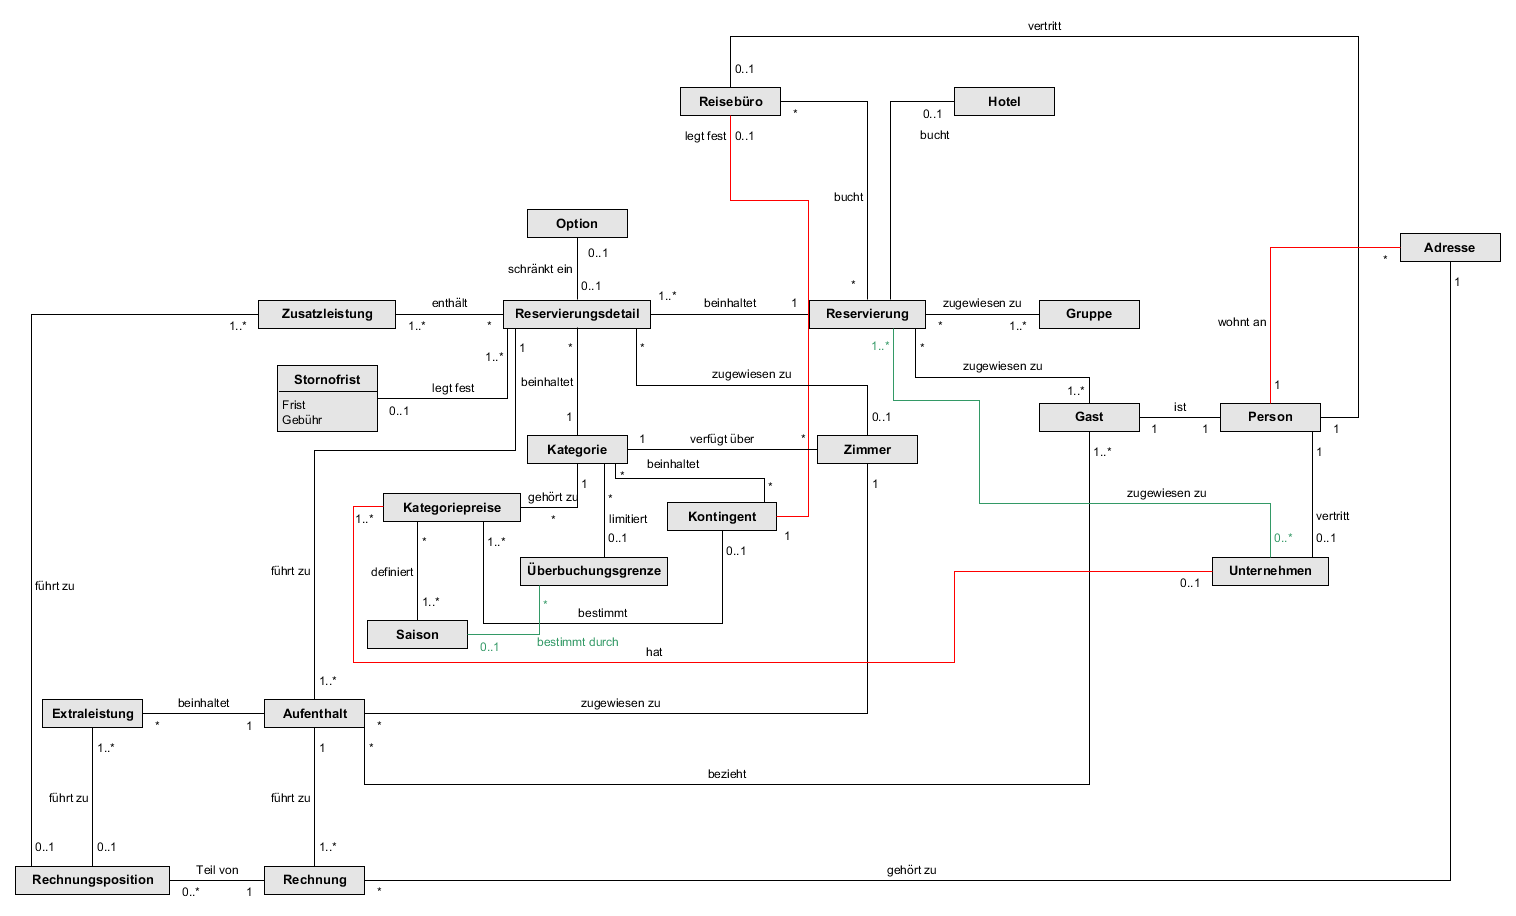
\includegraphics[width=0.6\textheight,angle=-89]{./assets/model_light.png}}
            \caption{Überblick des Domänenmodells ohne Attribute}\label{domainmodel}
        \end{center}
    \end{figure}
    \newpage
    \section{Detailliertes Modell}
    \begin{figure}[ht!]
        \begin{center}
            \rotatebox{-1}{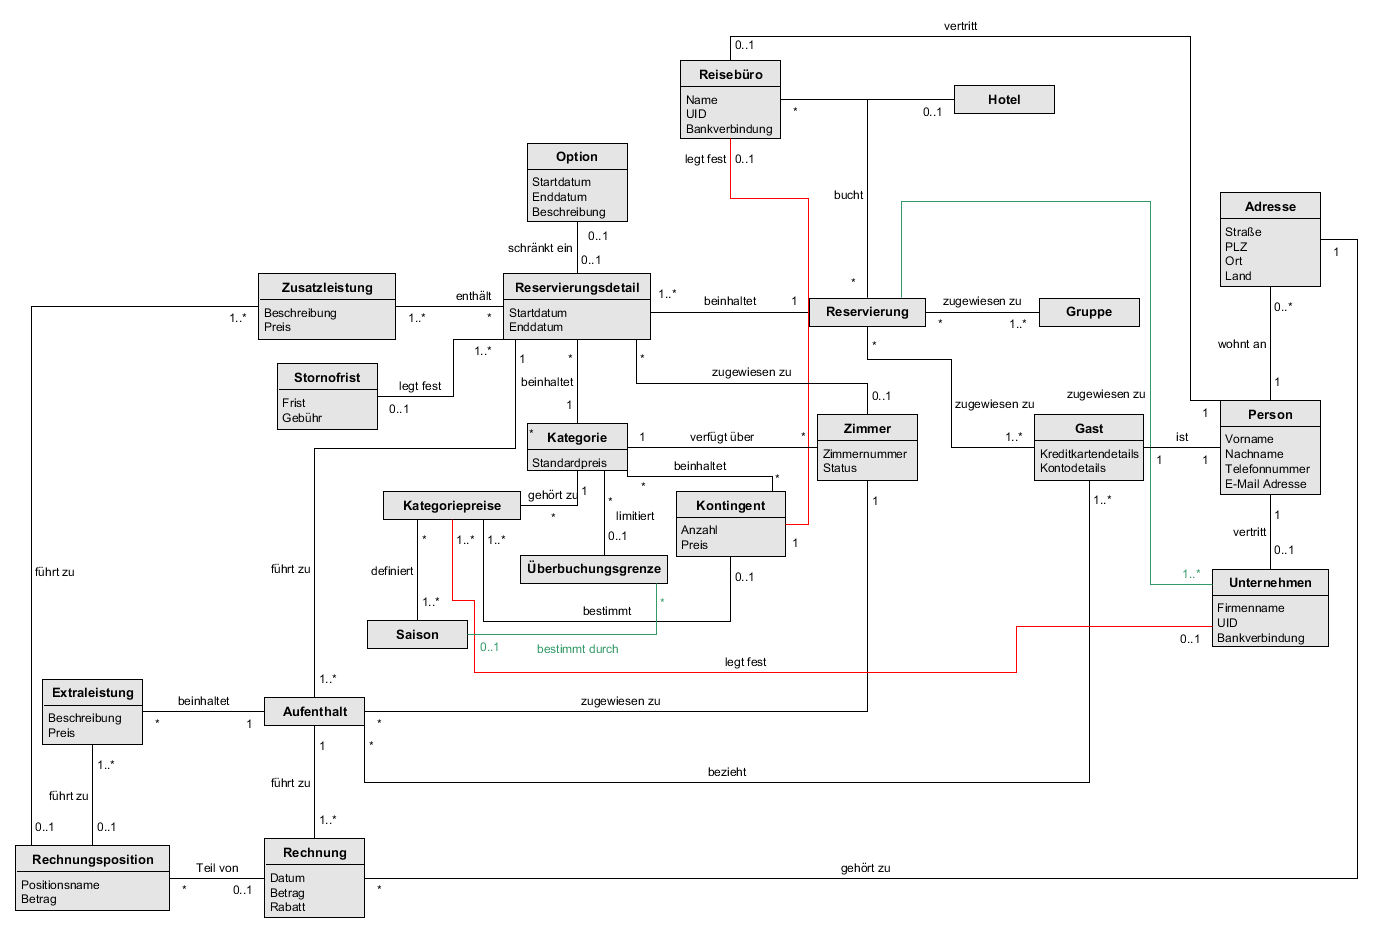
\includegraphics[width=0.8\textheight,angle=-89]{./assets/model.png}}
            \caption{Detailliertes Domänenmodell mit Attributen}\label{domainmodel_detail}
        \end{center}
    \end{figure}
    \subsection{Klasse 1}
    \subsection{Klasse 2}

    \section{Einschränkungen}
    Die Rechnungsnummer muss eine fortlaufende Zahl sein, die nicht geändert werden kann.

    \chapter{Dynamisches Modell}
    \section{Überblick}
    \section{Detaillierte Benutzungsfälle (Use Cases)}
        % detailed use cases main file
        \subfile{./content/usecases/detailed_overview_usecases.tex}

    \section{Objekt Lifecycles}

    \chapter{Nonfunktionale Anforderungen  }
    \section{Regeln}
        \subfile{./content/nonfunktionaleAnforderungen/Regeln.tex}
    \section{Usability}
        \subfile{./content/nonfunktionaleAnforderungen/Usability.tex}
    \section{Zuverlässigkeit}
        \subfile{./content/nonfunktionaleAnforderungen/Zuverlässigkeit.tex}
    \section{Performanz}
        \subfile{./content/nonfunktionaleAnforderungen/Performanz.tex}
    \section{Unterstützbarkeit}
        \subfile{./content/nonfunktionaleAnforderungen/Unterstützbarkeit.tex}
    \section{Online Benutzerdokumentation und Help System}
        \subfile{./content/nonfunktionaleAnforderungen/OnlineBenutzerdokumentationUndHelpSystem.tex}
    \section{zugekaufte Komponenten}
        \subfile{./content/nonfunktionaleAnforderungen/ZugekaufteKomponenten.tex}
    \section{Schnittstellen}
    \subsection{Benutzerschnittstellen}
        \subfile{./content/nonfunktionaleAnforderungen/Benutzerschnittstellen.tex}
    \subsection{Softwareschnittstellen}
        \subfile{./content/nonfunktionaleAnforderungen/Softwareschnittstellen.tex}
    \subsection{Kommunikationsschnittstellen}
        \subfile{./content/nonfunktionaleAnforderungen/Kommunikationsschnittstellen.tex}
    \section{zusätzliche Lizenzierungen}
        \subfile{./content/nonfunktionaleAnforderungen/ZusätzlicheLizenzierung.tex}
    \section{Copyright und andere rechtliche Anforderungen}
        \subfile{./content/nonfunktionaleAnforderungen/CopyrightUndAndereRechtlicheAnforderungen.tex}
    \section{Anzuwendende Standards}
        \subfile{./content/nonfunktionaleAnforderungen/AnzuwendendeStandards.tex}

    \chapter{Iterationsplan (Timeboxes)}
    \section{Überblick}
        Alle zuvor definierten Use Cases wurden von jedem Teammitglied auf einer Skala von 1 bis 10 in 3 Kategorien
        bewertet. 10 steht für eine hohe Relevanz. Von jeder Kategorie wurde das arithmetische Mittel berechnet
        und anschließend in der Spalte 'Gesamt' summiert.
        Die Kategorien haben folgende Bedeutung:
        \begin{enumerate}
            \item Risiko: Komplexität des Use Cases, Team Know How, Technologie.
            \item Architekturrelevanz: Ist der Use Case relevant für die Architektur(-entscheidung)?
            \item Benutzerrelevanz: Ist der Benutzer an einer frühen Realisierung des Use Cases interessiert?
        \end{enumerate}
        \begin{longtable}{|l|l|l|l|l|}
            \hline
                                         & Risiko & Architektur & Benutzer & Gesamt \\ \hline
            Reservierung Individualgast  & 8,25              & 9,75                   & 10                  & 28     \\
            CheckInMitreservierung       & 7,25              & 9,75                   & 10                  & 27     \\
            CheckOut                     & 7                 & 8,75                   & 9,5                 & 25,25  \\
            Walk in                      & 7,75              & 6,5                    & 8,75                & 23     \\
            Zimmerzuteilung              & 5,75              & 7,5                    & 7,75                & 21     \\
            Rechnung erstellen           & 4,75              & 8                      & 7,75                & 20,5   \\
            Rechnung legen               & 5,5               & 6,75                   & 7                   & 19,25  \\
            Reservierung Unternehmen     & 5,5               & 6,5                    & 7                   & 19     \\
            Rechnung teilen              & 5,75              & 6,5                    & 5,25                & 17,5   \\
            Reservierung stornieren      & 4,75              & 6                      & 6,5                 & 17,25  \\
            Reservierung Optionen        & 4,25              & 5,25                   & 7,5                 & 17     \\
            Zwischenrechnung erstellen   & 5                 & 6,25                   & 5,75                & 17     \\
            Rechnung stornieren          & 4,25              & 6                      & 6                   & 16,25  \\
            Reservierung ändern          & 4,25              & 4,75                   & 7,25                & 16,25  \\
            Individualgast anlegen       & 3,75              & 5,25                   & 6,75                & 15,75  \\
            Kassenabschluss              & 4,5               & 5                      & 6                   & 15,5   \\
            Rechnungsposition stornieren & 4,25              & 5,25                   & 6                   & 15,5   \\
            Zimmer wechseln              & 4,5               & 4,75                   & 5,75                & 15     \\
            Extraleistungen buchen       & 4                 & 5,25                   & 5,25                & 14,5   \\
            Rechnungen zusammenlegen     & 4,5               & 5                      & 4,75                & 14,25  \\
            Stammdaten ändern            & 4                 & 4,75                   & 4,75                & 13,5   \\
            Zimmerstatus setzen          & 3,75              & 4,5                    & 5,25                & 13,5   \\
            Tagesabschluss erstellen     & 3,5               & 3,5                    & 5,5                 & 12,5   \\
            Aufenthaltsdauer ändern      & 3,25              & 3,75                   & 4,5                 & 11,5   \\
            Kassastornierung             & 2,75              & 4                      & 4                   & 10,75  \\
            Akonto buchen                & 3                 & 2,75                   & 4,75                & 10,5   \\
            Monatsabschluss erstellen    & 3                 & 3,75                   & 3,5                 & 10,25  \\
            Jahresabschluss erstellen    & 2,5               & 3,25                   & 3                   & 8,75
            \hline
        \end{longtable}


    \section{1. Timebox}
        \subfile{./content/timebox/timebox1.tex}

    \section{2. Timebox}
        \subfile{./content/timebox/timebox2.tex}

    \section{3. Timebox}
        \subfile{./content/timebox/timebox3.tex}

    \chapter{Glossar}
        \subfile{./content/glossar/glossar.tex}

    %\chapter*{Eidesstattliche Erklärung}
    %\addcontentsline{toc}{chapter}{Eidesstattliche Erklärung}
    %Ich erkläre hiermit an Eides statt, dass ich die vorliegende Arbeit selbstständig und ohne Benutzung anderer als der angegebenen Hilfsmittel angefertigt habe. Die aus fremden Quellen direkt oder indirekt übernommenen Stellen sind als solche kenntlich gemacht. Die Arbeit wurde bisher weder in gleicher noch in ähnlicher Form einer anderen Prüfungsbehörde vorgelegt und auch noch nicht veröffentlicht.

    %\vspace{3cm}
    %\noindent
    %Dornbirn, am [Tag. Monat Jahr anführen]\hfill [Vor- und Nachname Verfasser/in]

\end{document}
